\documentclass[a4paper,USenglish]{article}
\usepackage[T1]{fontenc}
\usepackage[utf8]{inputenc}
\usepackage{amsmath, amsfonts, amssymb,mathtools,nicefrac, amsthm}
\usepackage{tikz}
\usetikzlibrary{calc}
\usetikzlibrary{patterns}
\usetikzlibrary{decorations.pathreplacing}
\usetikzlibrary{fadings}

\begin{document}

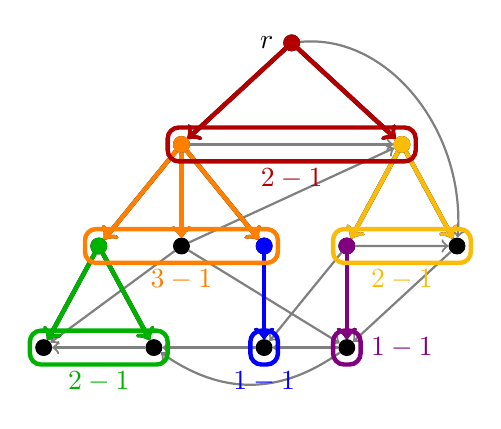
\begin{tikzpicture}[mynode/.style={circle, minimum size = 2mm, inner sep = 0pt, draw, fill}, xscale = 0.35, yscale=0.43]
	\node[mynode, label=left:$r$] (R) at (0,0){};
	\node[mynode] (A) at (-4,-3){};
	\node[mynode] (B) at  (4,-3){};
	
	\node[mynode] (C) at (-7,-6){};
	\node[mynode] (D) at  (-4,-6){};
	\node[mynode] (E) at  (-1,-6){};
	\node[mynode] (F) at  (2,-6){};
	\node[mynode] (G) at  (6,-6){};
	
	\node[mynode] (H) at (-9,-9){};
	\node[mynode] (I) at (-5,-9){};
	\node[mynode] (J) at (-1,-9){};
	\node[mynode] (K) at (2,-9){};
	
	%other arcs
	\draw[thick,->,black!50!white] (A)--(B);
	\draw[thick,->,black!50!white] (D)--(B);
	\draw[thick,->,black!50!white] (D)--(K);
	\draw[thick,->,black!50!white] (I)--(H);
	\draw[thick,->,black!50!white] (J)--(I);
	\draw[thick,->,black!50!white] (D)--(H);
	\draw[thick,->,black!50!white] (K)--(J);
	\draw[thick,->,black!50!white] (F)--(J);
	\draw[thick,->,black!50!white, bend left=30] (K) to (I);
	\draw[thick,->,black!50!white] (F)--(G);
	\draw[thick,->,black!50!white] (G)--(K);
	\draw[thick,->,black!50!white, bend left=50] (R) to (G);
	
	%arborescence
	\draw[ultra thick,->] (R)--(A);
	\draw[ultra thick,->] (R)--(B);
	
	\draw[ultra thick,->] (A)--(C);
	\draw[ultra thick,->] (A)--(D);
	\draw[ultra thick,->] (A)--(E);
	\draw[ultra thick,->] (B)--(F);
	\draw[ultra thick,->] (B)--(G);
	
	\draw[ultra thick,->] (C)--(H);
	\draw[ultra thick,->] (C)--(I);
	\draw[ultra thick,->] (E)--(J);
	\draw[ultra thick,->] (F)--(K);
	
	%arborescence
	\draw[ultra thick,->, red!70!black] (R)--(A);
	\draw[ultra thick,->, red!70!black] (R)--(B);
	
	\draw[ultra thick,->, orange] (A)--(C);
	\draw[ultra thick,->, orange] (A)--(D);
	\draw[ultra thick,->, orange] (A)--(E);
	\draw[ultra thick,->, yellow!50!orange] (B)--(F);
	\draw[ultra thick,->, yellow!50!orange] (B)--(G);
	
	\draw[ultra thick,->, green!70!black] (C)--(H);
	\draw[ultra thick,->, green!70!black] (C)--(I);
	\draw[ultra thick,->, blue] (E)--(J);
	\draw[ultra thick,->, blue!50!red] (F)--(K);
	
	\node[mynode, draw=red!70!black, fill=red!70!black] at (0,0){};
	\draw[ultra thick, rounded corners, draw=red!70!black] (-4.5,-3.5) rectangle (4.5,-2.5);
	
	\node[mynode,draw=orange, fill = orange] at (-4,-3){};
	\draw[ultra thick, rounded corners, draw=orange] (-7.5,-6.5) rectangle (-0.5,-5.5);
	\node[mynode, draw=yellow!50!orange, fill=yellow!50!orange] (B) at  (4,-3){};
	\draw[ultra thick, rounded corners, draw=yellow!50!orange] (1.5,-6.5) rectangle (6.5,-5.5);
	
	\node[mynode, draw=green!70!black, fill=green!70!black] at (-7,-6){};
	\draw[ultra thick, rounded corners, draw=green!70!black] (-9.5,-9.5) rectangle (-4.5,-8.5);
	\node[mynode, draw=blue, fill=blue] (E) at  (-1,-6){};
	\draw[ultra thick, rounded corners, draw=blue] (-1.5,-9.5) rectangle (-0.5,-8.5);
	\node[mynode, draw=blue!50!red, fill=blue!50!red] (F) at  (2,-6){};
	\draw[ultra thick, rounded corners, draw=blue!50!red] (1.5,-9.5) rectangle (2.5,-8.5);
	
	\node at (0,-4){$\color{red!70!black}2-1$};
	\node at (-4,-7){$\color{orange}3-1$};
	\node at (4,-7){$\color{yellow!50!orange}2-1$};
	\node at (-7,-10){$\color{green!70!black}2-1$};
	\node at (-1,-10){$\color{blue}1-1$};
	\node at (4,-9){$\color{blue!50!red}1-1$};
\end{tikzpicture}

\end{document}